\chapter{Method}

Some of the methods used to produce the results in Chapters \ref{chapter:spectroscopy} and \ref{chapter:imaging} are discussed in this chapter.  Spectra fitting, used for separating contributions of semi-resolved fluorescence peaks, is discussed in Sec. \ref{sec:fitting}.  Background signals are discussed in Sec. \ref{sec:bgs} with the purpose of optimizing signal-to-background for imaging of small numbers of Ba atoms.

\section{Fitting of Spectra}
\label{sec:fitting} %appendix:fitting

The spectra of Ba\textsuperscript{+} deposits in SXe are described in detail for green excitation ($\sim$540-590~nm) in Sec. \ref{sec:fluorescence}, and for blue excitation ($\sim$460-490~nm) in Sec. \ref{sec:BaPlus}.  Chi-square fitting to these spectra using ROOT is described in this section.  In most circumstances, the different fluorescence peaks in a spectrum overlap somewhat.  Thus it was necessary to fit the fluorescence spectra with a sum of peak-specific fit functions in order to extract peak heights and integrals.  Gaussians, Lorentzians and asymmetric functions were used, depending on the best match to a specific peak.  Fit function parameters are not intended to determine physical properties in this thesis.  Rather, fits are used to track fluorescence peak amplitudes under various circumstances, e.g., in excitation spectra (Sec. \ref{sec:fluorescence},\ref{sec:BaPlus}), annealing (Sec. \ref{sec:tempanneal}), and bleaching (Sec. \ref{sec:bleaching}).  When extracting fluorescence peak amplitudes from spectra, shape parameters (center and widths) were fixed, and amplitudes were allowed to float.  Determination of those fixed shape parameters was done prior, by fitting spectra where the peak of interest is strong and letting all parameters float.
%These were used, e.g., in excitation spectra, annealing, and bleaching curves for different peaks.

%The center and width parameters of the fit functions were fixed, while the amplitudes were the free fitting parameters.  Center and width parameters for each peak were determined by fitting spectra where that peak is relatively large.  Some fine-tuning was done to match slightly different shapes resulting from different excitation wavelengths.

\subsection{Fitting Spectra with Green Excitation}
\label{subsec:fitgrn} %sec:fitgrn

\begin{figure} %[H]
        \centering
                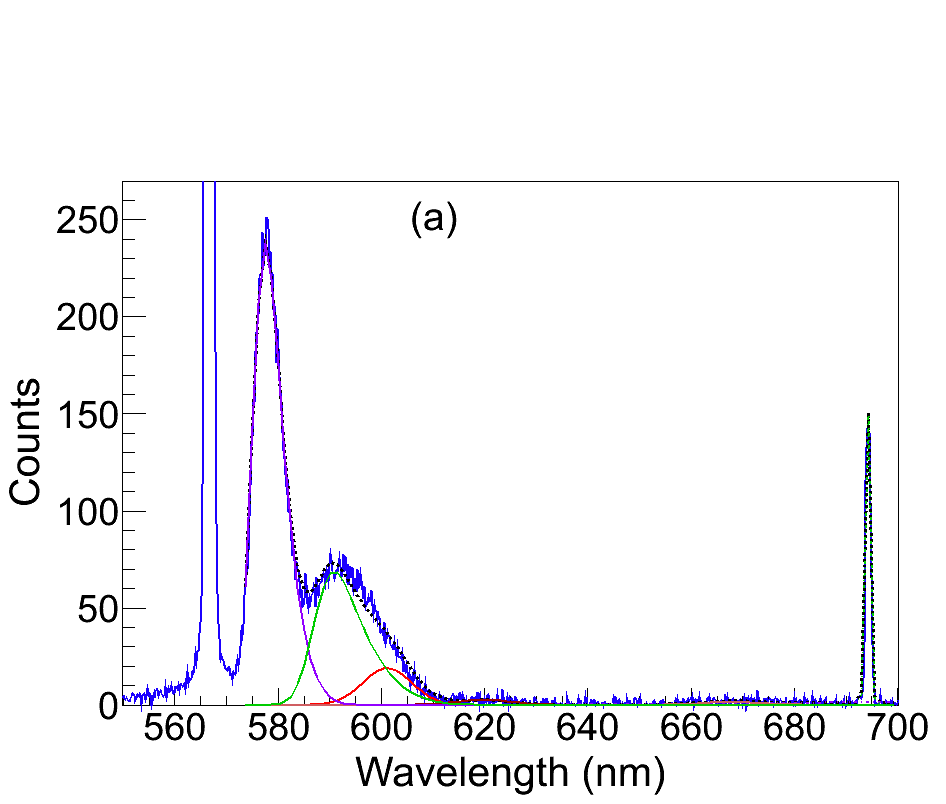
\includegraphics[width=.5\textwidth]{figures/spectra_fit_a.png}
                ~
                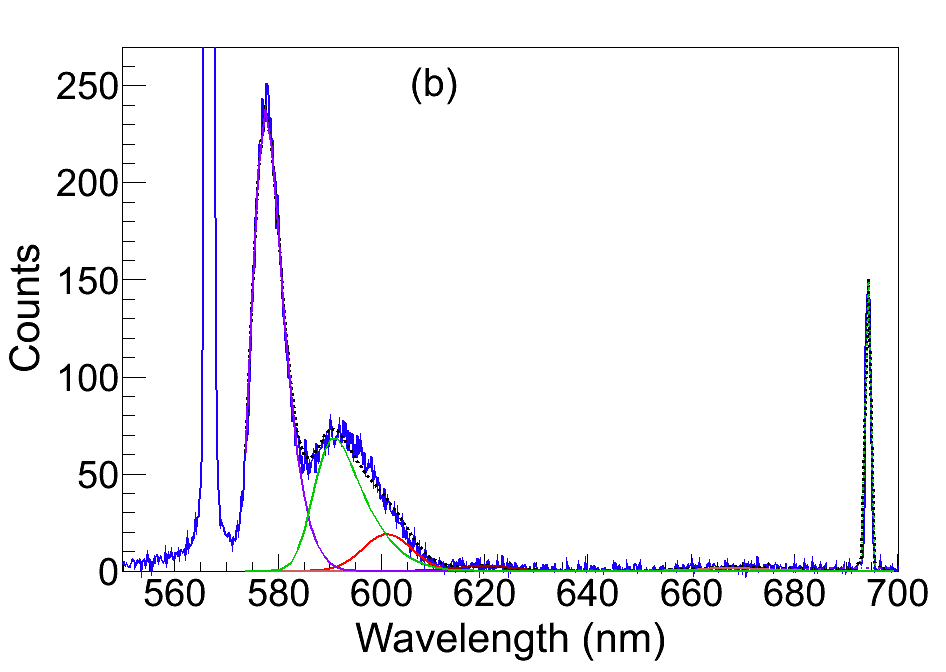
\includegraphics[width=.5\textwidth]{figures/spectra_fit_b.png}
                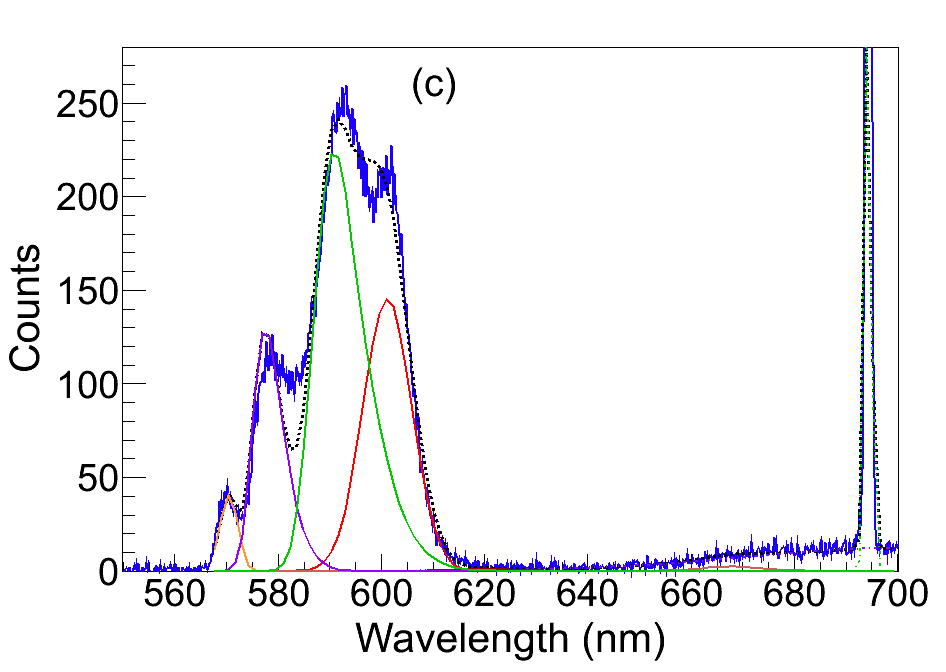
\includegraphics[width=.5\textwidth]{figures/spectra_fit_c.png}
                ~
                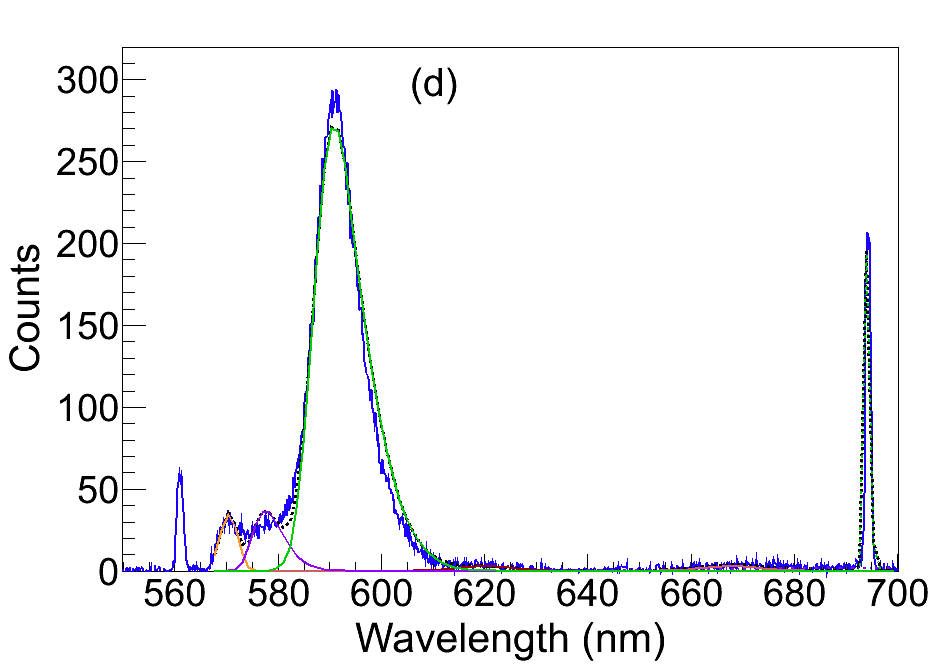
\includegraphics[width=.5\textwidth]{figures/spectra_fit_d.png}
                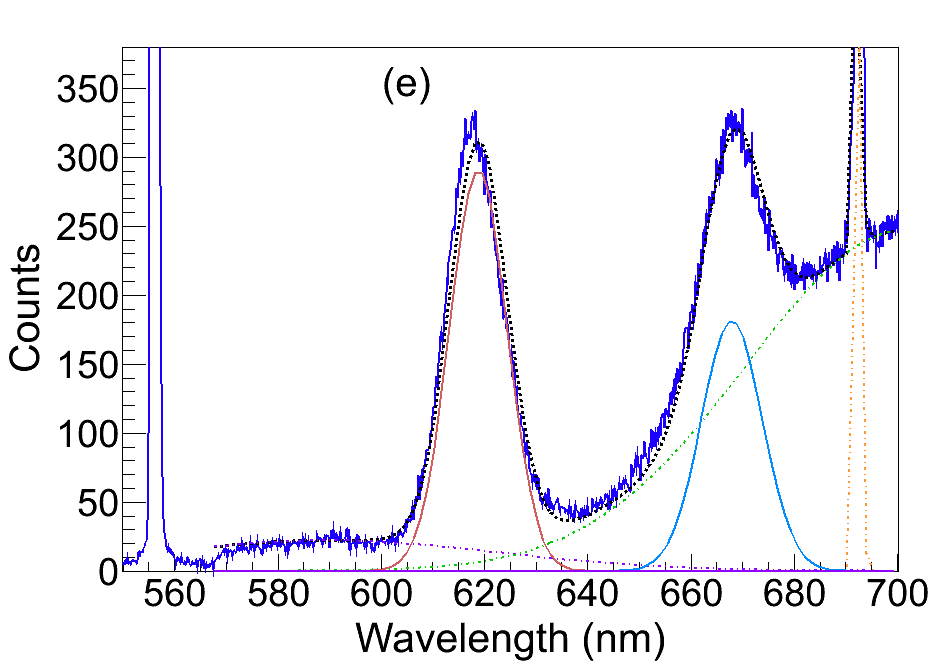
\includegraphics[width=.5\textwidth]{figures/spectra_fit_e.png}
                ~
                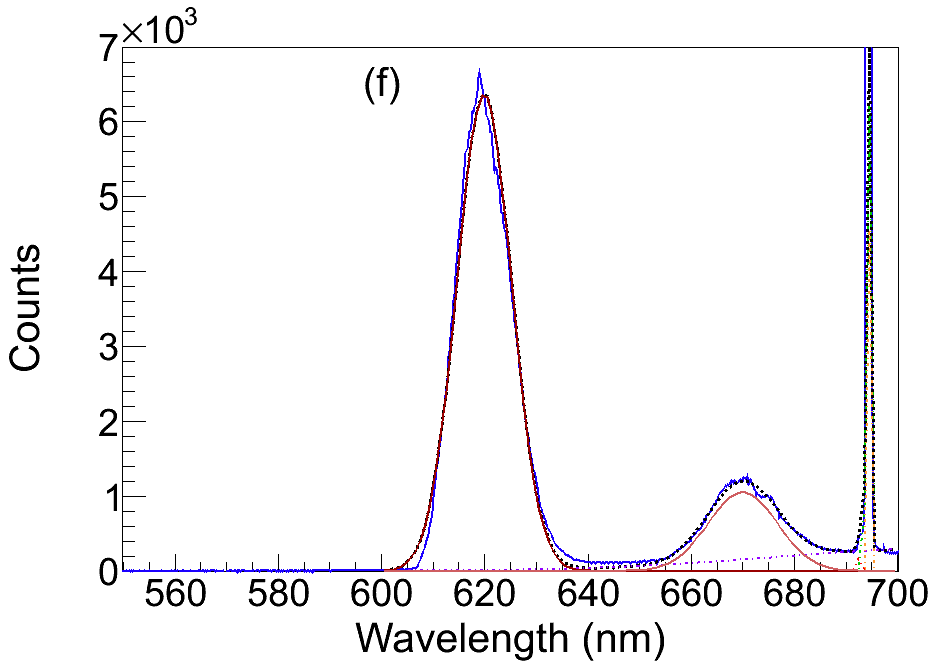
\includegraphics[width=.5\textwidth]{figures/spectra_fit_f.png}
                \caption{Example fits to spectra of Ba\textsuperscript{+} deposits with green excitation at (a) 567.3~nm, (b) 566.6~nm, (c) 563.4~nm, (d) 561.0~nm, (e) 555.9~nm, and (f) 546.3~nm.  Laser scatter can be seen in the lower wavelengths for some figures, especially in (b) where it is on the edge of the Raman filter cutoff.}
\label{fig:specFitsGrn}
\end{figure}

Example fits to spectra for several different green excitation wavelengths are shown in Fig. \ref{fig:specFitsGrn}.  To incorporate the tail in the shape of the 577- and 591-nm peaks, an asymmetric function of the form $A(1+$erf$(\frac{x-a}{\sigma_{1}})(1-$erf$(\frac{x-a}{\sigma_{2}}))$ was used, where $a$ is the fixed center-defining parameter, $\sigma_{1}$ and $\sigma_{2}$ are fixed left and right width parameters, and $A$ is the free amplitude parameter.  The function erf() is an error function.  The 570-, 601-, 619-, and 670-nm peaks were fit with Gaussian functions with fixed standard deviation ($\sigma$) of 1.7~nm, 4.7~nm, 5.3~nm, and 6.7~nm, respectively.  Rather than attempting frame-by-frame background subtractions, additional Gaussians were fit to the broad and sharp background fluorescence.  Two broad Gaussians centered at around 590~nm and 702~nm, and one sharp Gaussian near 693~nm, were chosen by fitting spectra of Xe-only deposits.  These backgrounds and their excitation spectra are discussed in Sec. \ref{sec:bgs}.  The full fit, i.e. the sum of each contributing peak fit, is the dotted black line.  Though the shapes do not match perfectly for all excitation wavelengths, the fits still follow the peak amplitudes well.  Ba emission and excitation spectra results are discussed in Sec. \ref{sec:fluorescence}.

\subsection{Fitting Spectra with Blue Excitation}
\label{subsec:fitblu} %sec:fitblu

Example fits to spectra for several different blue excitation wavelengths are shown in Fig. \ref{fig:specFitsBlu}.  Gaussian functions were used for the 532-, 568-, and 575-nm peaks with standard deviations ($\sigma$) of 2.4~nm, 5.0~nm, and 0.7~nm, respectively.  Lorentzian functions were used for the 553-, 592-, 635-, and 669-nm peaks with half width at half maxima ($\gamma$) of 1.7~nm, 13.8~nm, 10.4~nm. and 9.1~nm, respectively.  Similar to spectra with green excitation, the background components were fit with two broad Gaussians centered at 546.0~nm and 703.3~nm, with respective $\sigma$ of 49.0~nm and 30.5~nm, as well as one sharp Gaussian centered at 693.4~nm peak with a $\sigma$ of 0.5~nm.  The fits for excitation around 478~nm (e.g., (c)) are not quite right, mainly due to a shift in the central value of the 592-nm peak.  However, fit values still follow respective peaks heights well.  The sharp 522- and 575-nm peaks are seen in (c), though the 522-nm peak is left out of the fitting range since it sits on the edge of the Raman filter cutoff.   These spectra are discussed in Sec. \ref{sec:BaPlus}.

\begin{figure} %[H]
        \centering
                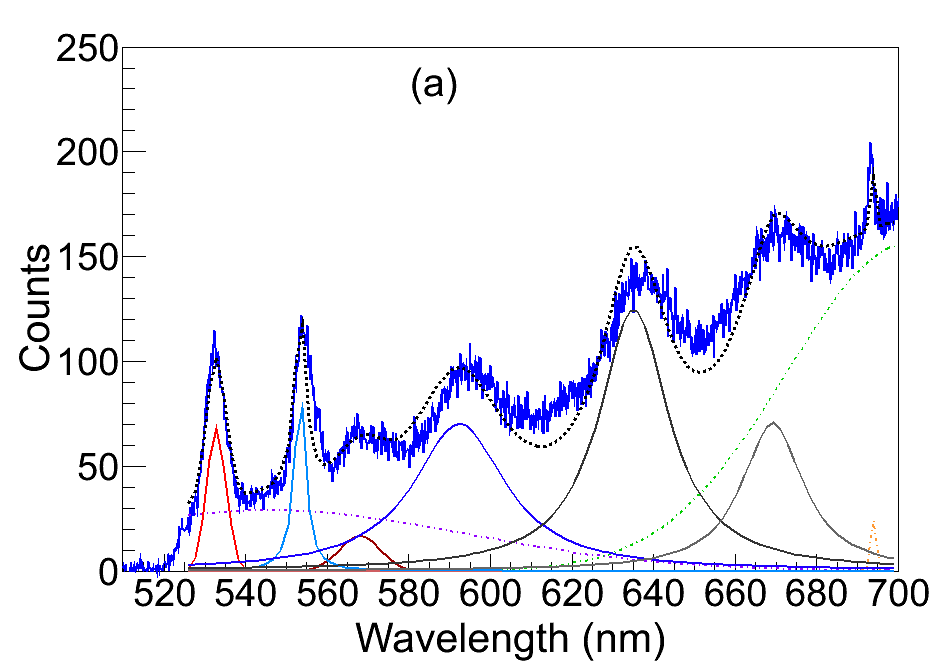
\includegraphics[width=.5\textwidth]{figures/spectra_blu_fit_a.png}
                ~
                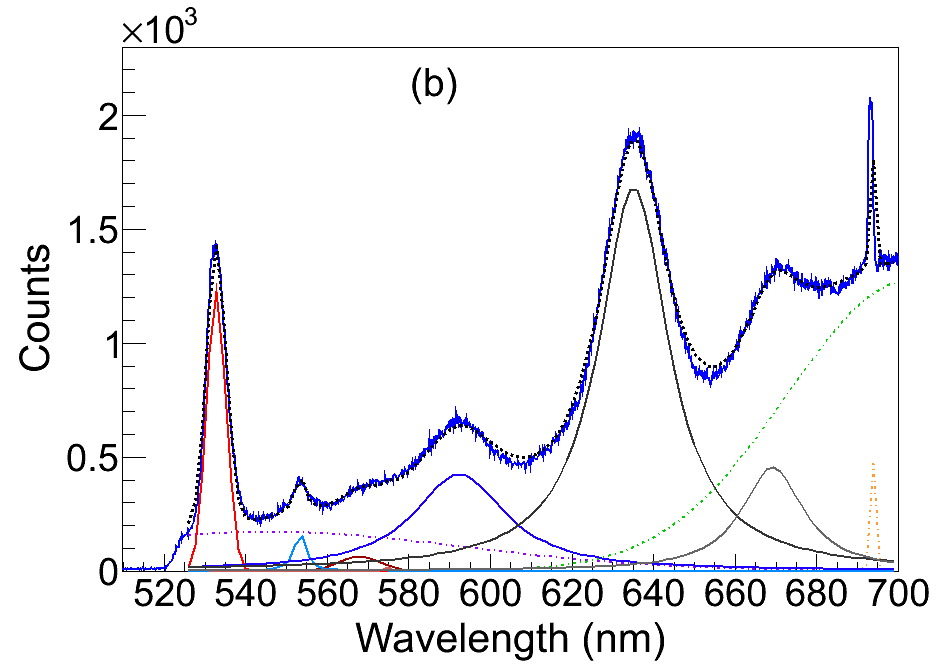
\includegraphics[width=.5\textwidth]{figures/spectra_blu_fit_b.png}
                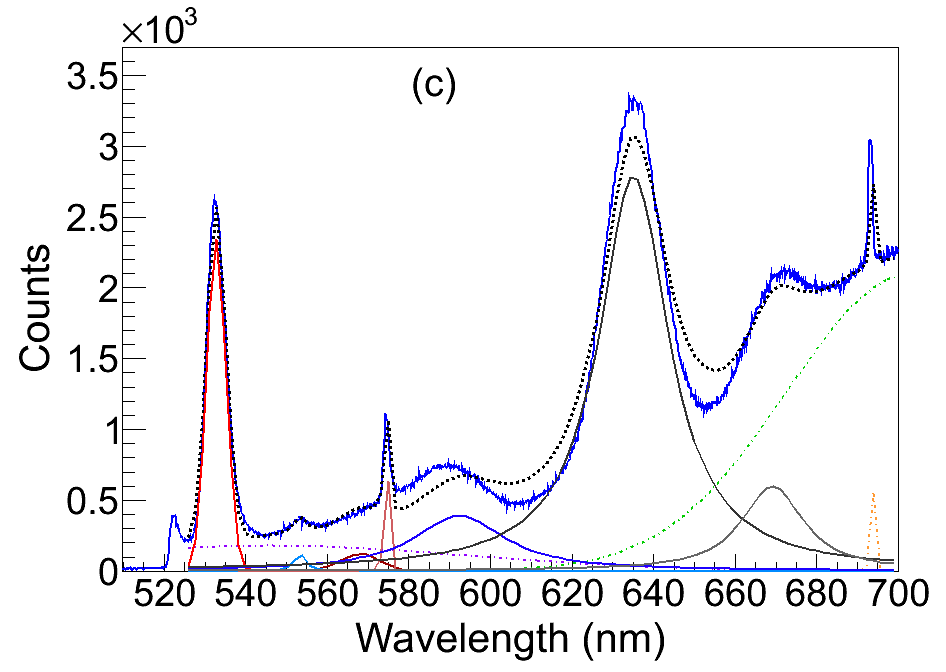
\includegraphics[width=.5\textwidth]{figures/spectra_blu_fit_c.png}
                ~
                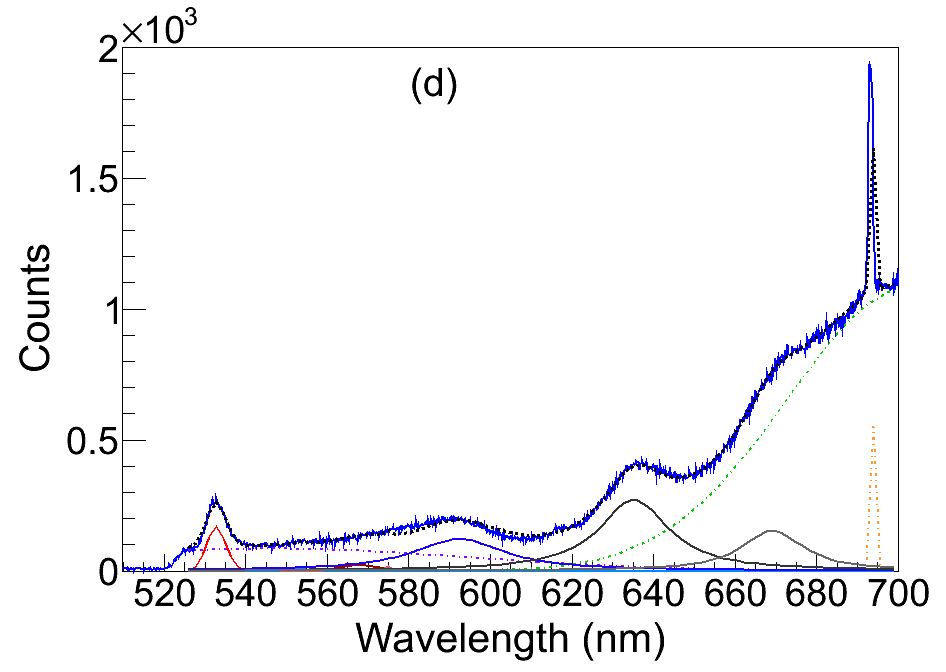
\includegraphics[width=.5\textwidth]{figures/spectra_blu_fit_d.png}
                \caption{Example fits to spectra of Ba\textsuperscript{+} deposits with blue excitation at (a) 461.7~nm, (b) 468.2~nm, (c) 478.3~nm, and (d) 488.2~nm.}
\label{fig:specFitsBlu}
\end{figure}

\section{Background Spectra}
\label{sec:bgs} %appendix:bgs

The sharp and broad background discussed in Sec. \ref{subsec:fitgrn} is mainly due to Cr\textsuperscript{3+} impurity ions in the sapphire window.  A spectrum of this fluorescence with 562~nm excitation is shown in Fig. \ref{fig:Cr}a.  The strong, sharp peak around 693~nm is a well-known $^{2}E$ - $^{4}A_{2}$ emission in the $d^{3}$ configuration of Cr\textsuperscript{3+} impurities in the sapphire bulk \cite{SapphireRlines1964,SapphireRlines2010}.  An excitation spectrum for this peak is shown in Fig. \ref{fig:Cr}b over the range all three dyes R6G, R110, and C480, using one of the sapphire windows with higher Cr\textsuperscript{3+} content.  Multiple features are observed in the excitation spectrum, obtained by integrating the 693-nm peak fit (Sec. \ref{sec:fitting}) vs. excitation wavelength.  The broad absorption in the green/yellow, peaking around 550~nm, with vibrational peaks on the red tail, agree with well understood features in the spectrum of Cr\textsuperscript{3+} in sapphire, including three sharp peaks in the blue at 468.4, 474.8, and 476.5~nm \cite{SapphireFord,SapphireMcclure}.  In addition to the 693-nm peak, a weaker and much broader emission is observed, along with three weak peaks in the 615-635~nm region.  Excitation spectra for these fluorescence components are shown in Fig. \ref{fig:CrBroad} for the R6G dye range.  In this experiment, the laser was de-focused to about w = 200~$\mu$m, and the emission observed had contribution of the surface background as well as the bulk sapphire emission.  The surface background is negligible for the prominent 693-nm peak.  However, the rising features of the surface background excitation spectrum near 600~nm and 567~nm (see below) can be seen in the excitation spectra of the weaker components (blue, and especially orange curves in Fig. \ref{fig:CrBroad}).  Nonetheless, observation of the same vibrational peaks as in the 693-nm peak excitation spectrum demonstrates that the broad emission and weak peaks in the 620 band-pass (Fig. \ref{fig:Cr}a) are also due to Cr\textsuperscript{3+} in the sapphire.  Commercially available c-plane quality sapphire windows contain low concentrations of Cr\textsuperscript{3+}.  Sample windows of 0.75" diameter and 0.02" thickness from a few companies were tested, and those from Meller Optics produced the lowest sapphire bulk emission in the 620-nm band-pass region.

% at 77~K

\begin{figure} %[H]
        \centering
                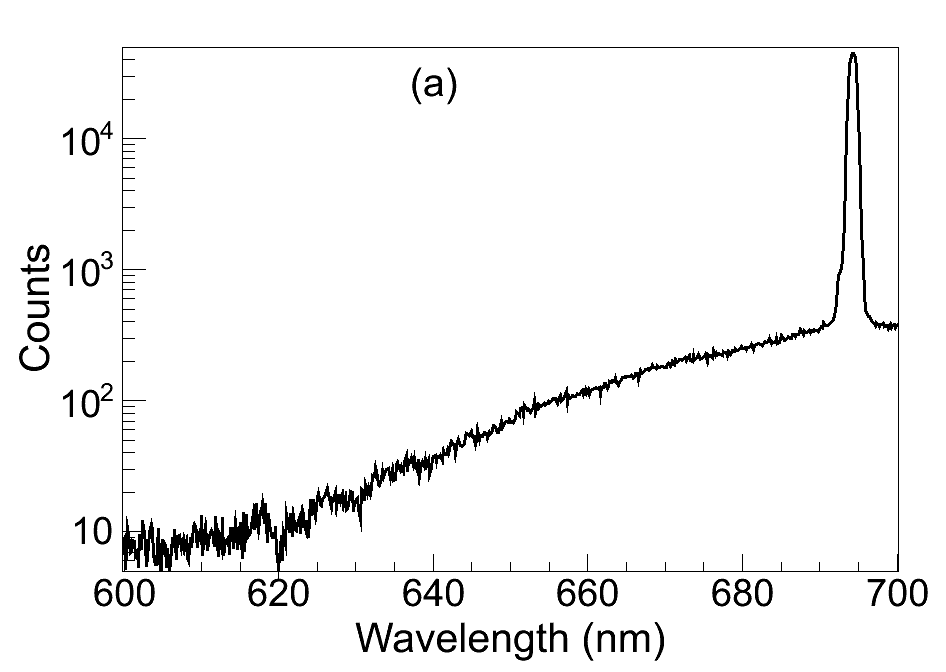
\includegraphics[width=.5\textwidth]{figures/Cr_a.png}
                ~
                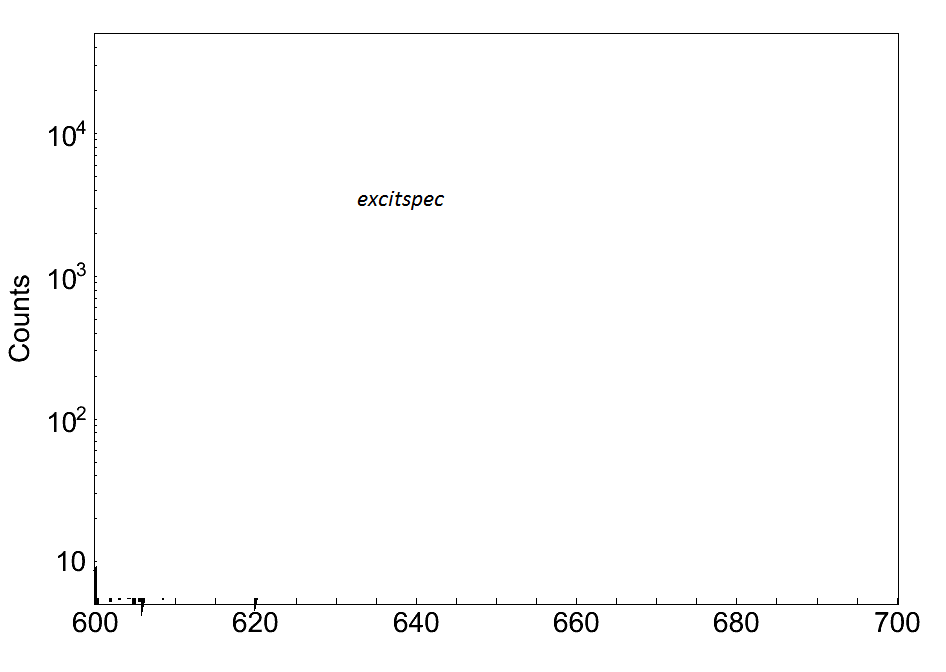
\includegraphics[width=.5\textwidth]{figures/Cr_b.png}
                \caption{(a) Sapphire bulk emission with 562-nm excitation at 11~K, and (b) excitation spectrum of the sharp 693-nm emission peak using three different laser dyes.  Due to different laser powers and exposure times, the R110 and R6G were scaled to match at their boundary.}
\label{fig:Cr}
\end{figure}

\begin{figure} %[H]
        \centering
                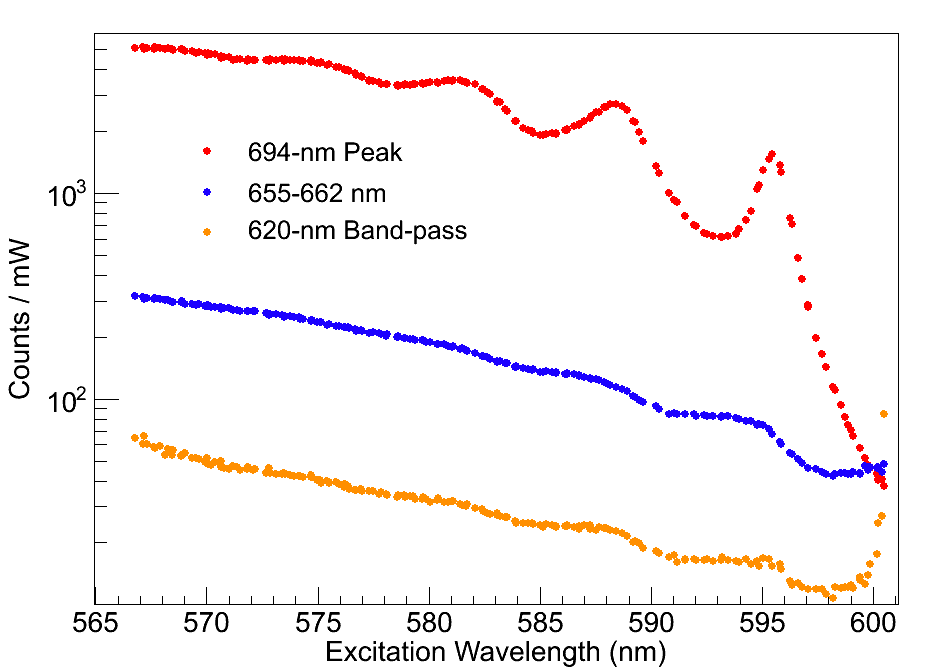
\includegraphics[width=.7\textwidth]{figures/Cr_broad.png}
                \caption{Excitation spectra for weaker sapphire bulk emissions (blue,orange) along with that of the strong 693-nm emission (red) at 11~K.}
        \label{fig:CrBroad}
\end{figure}

An additional background emission was observed from the surfaces of the window.  Its broad fluorescence is shown in Fig. \ref{fig:surfBG}a with a 610-nm Raman filter cutoff and 570.4~nm excitation, and its excitation spectrum is shown in Fig. \ref{fig:surfBG}b over the R6G dye range.  The nature of this emission has not been determined, however a few characteristics were identified.  One was that the emission increased as the window temperature was decreased, down to about 100~K where it remained flat down to 11~K, shown in Fig. \ref{fig:BGtempDependence}.  Another feature of the surface background is that it bleaches, i.e. is reduced during laser exposure.  In order to reduce this background in imaging experiments, as well as to reduce run-to-run variation in the background due to bleaching, the sapphire window was pre-bleached for at least half an hour at 100~K.  Decay of the surface background emission from a focused laser region, with intermittent observation during a pre-bleaching process, is shown in Fig. \ref{fig:surfBGbleach}.  For efficient pre-bleaching, the dye laser was usually tuned to 580.5~nm for higher laser power ($\sim$10~mW), although the bleaching data in Fig. \ref{fig:surfBGbleach} were taken with the dye laser at 570~nm ($\sim$0.1~mW) with the same laser power used in typical Ba imaging experiments.  During imaging experiments, frequent Xe-only deposits were made in order to track the surface background emission to establish proper background subtraction.

\begin{figure} %[H]
        \centering
                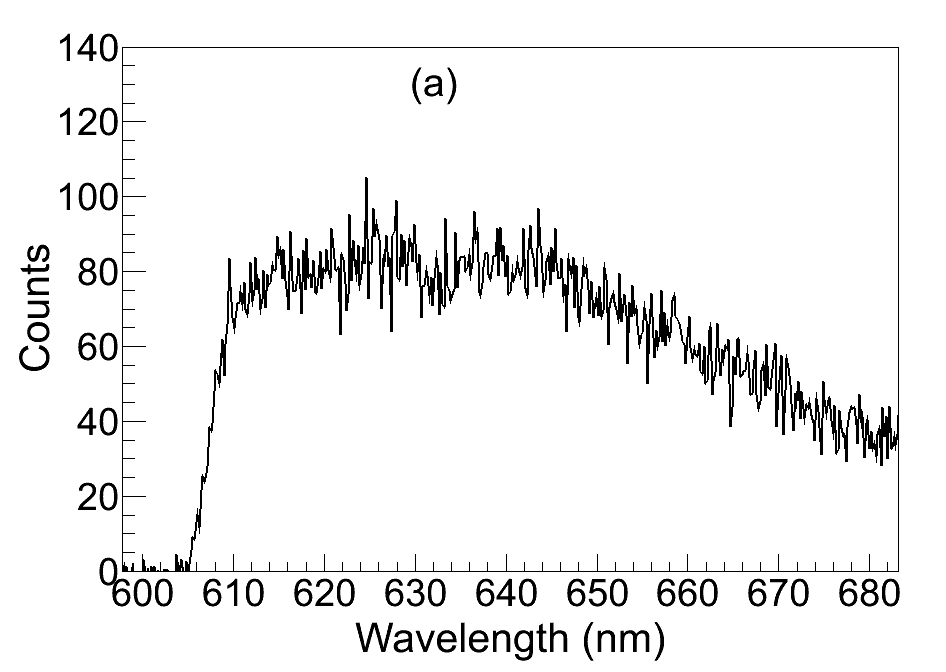
\includegraphics[width=.5\textwidth]{figures/surfaceBG_a.png}
                ~
                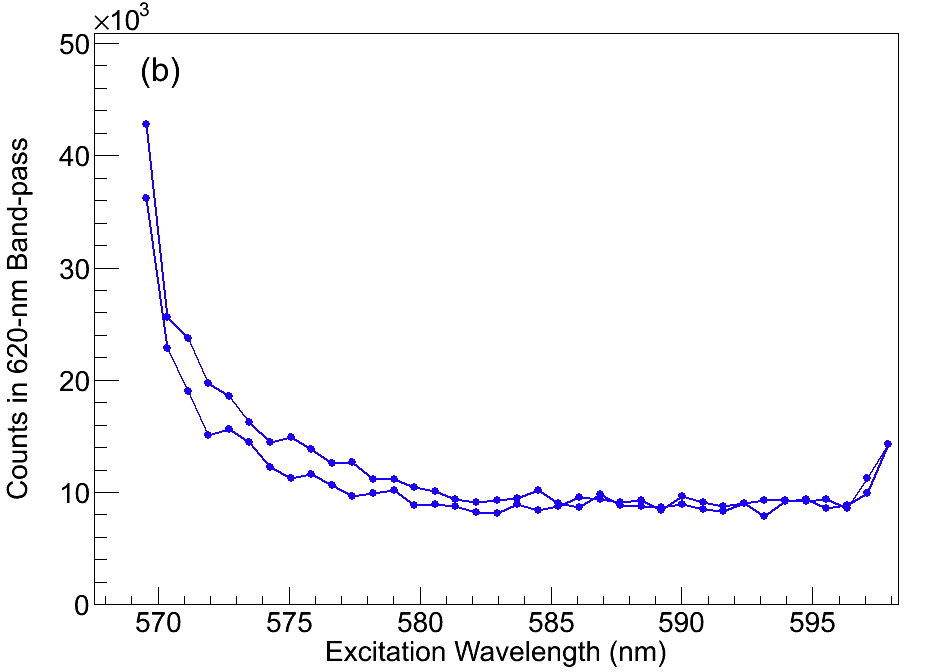
\includegraphics[width=.5\textwidth]{figures/surfaceBG_b.png}
                \caption{(a) Surface background emission spectrum w/ excitation at 570.5~nm, and (b) excitation spectrum in R6G dye range.  The sharp drop in (a) around 608~nm is the Raman filter cutoff.}
\label{fig:surfBG}
\end{figure}

%\begin{figure} %[H]
%        \centering
%                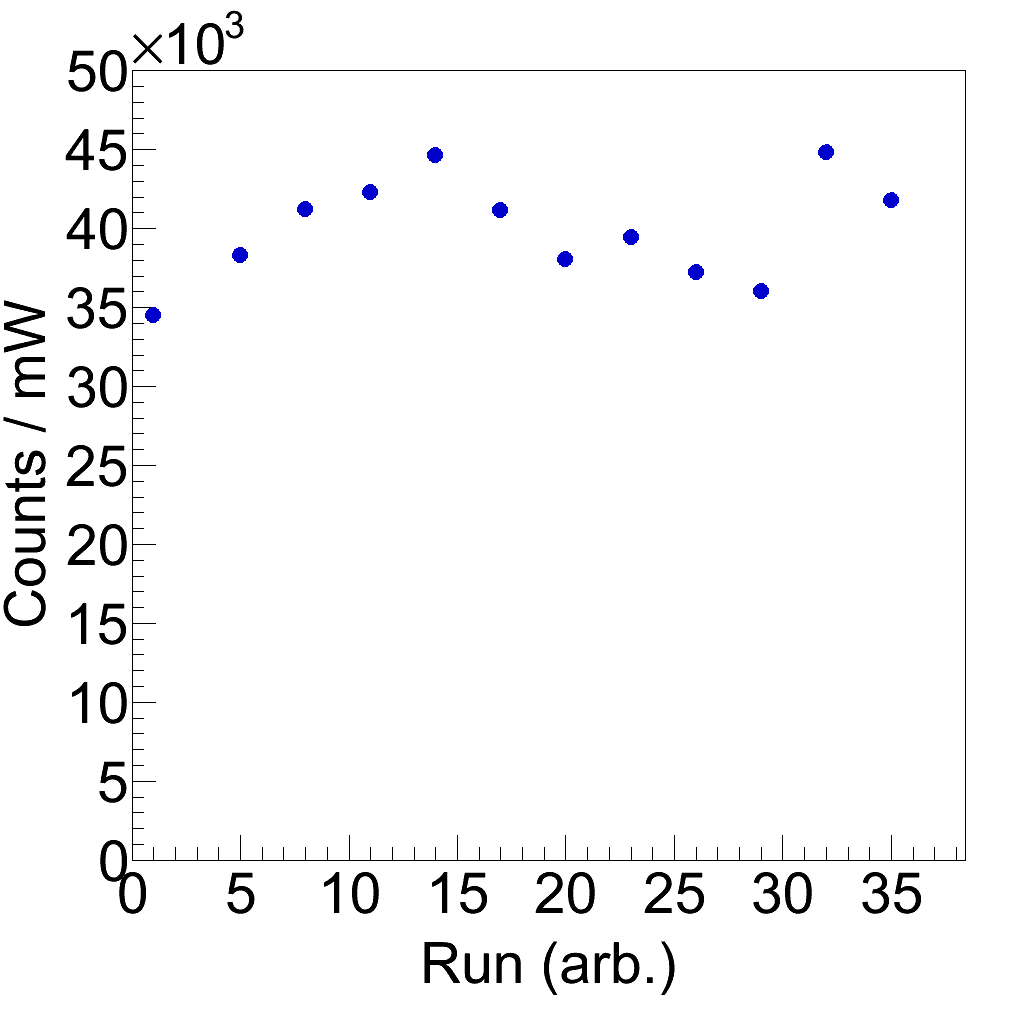
\includegraphics[width=.4\textwidth]{figures/xe_variation.png}
%                \caption{Background counts in focused laser region over the course of an experiment.}
%\label{fig:xevar}
%\end{figure}

%\emph{\color{gray}from results} Variation in the background level, dominated by the surface background, is shown in Fig. \ref{fig:xevar}.  Variation was most likely caused by drift of the laser position on the window, to regions of different historical bleaching.  Local variations are at the single-atom signal level, however positive signal after subtraction, even at the single-atom level, demonstrates that this variation is sufficiently low.

%Spacial variation in the background is especially cumbersome in a laser scanning experiment, as discussed in \ref{sec:scanning}. 

%speculation:    Given these behaviors, it is possible that the surface background is caused by a species which freezes to the window, or something which coats the window and fluoresces more at lower temperatures.  In either case, the bleaching could be explained by evaporation with laser heating, or by optical pumping of the species into a metastable state.

\begin{figure} %[H]
        \centering
                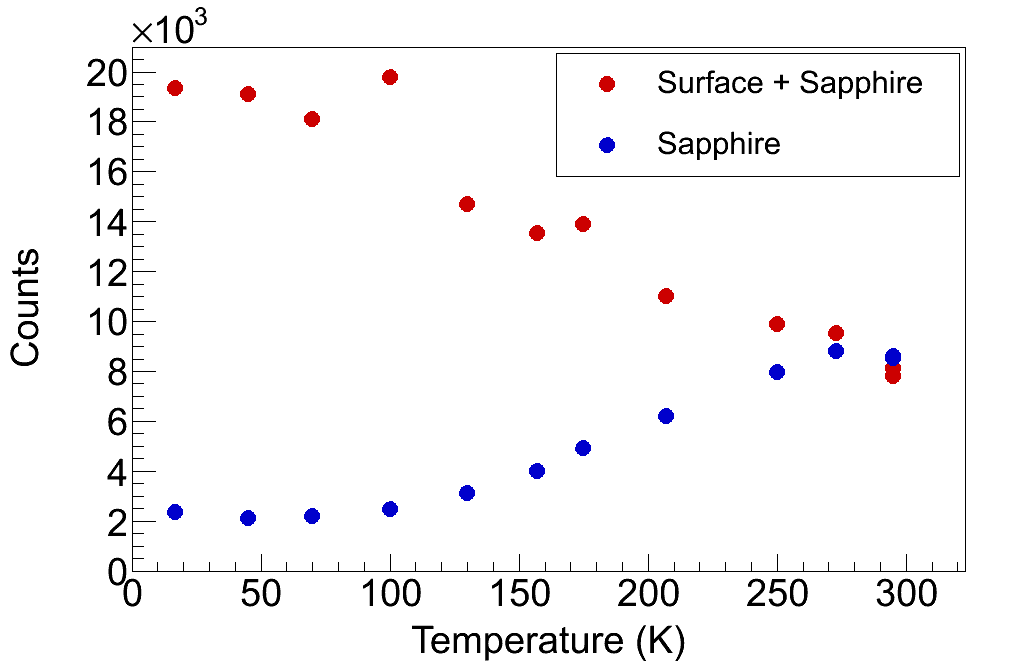
\includegraphics[width=.6\textwidth]{figures/bg_temp_dep.png}
                \caption{Temperature dependence of surface (red) and sapphire bulk (b) backgrounds. Fluorescence is observed through 620-nm band-pass filter.}
\label{fig:BGtempDependence}
\end{figure}

\begin{figure} %[H]
        \centering
                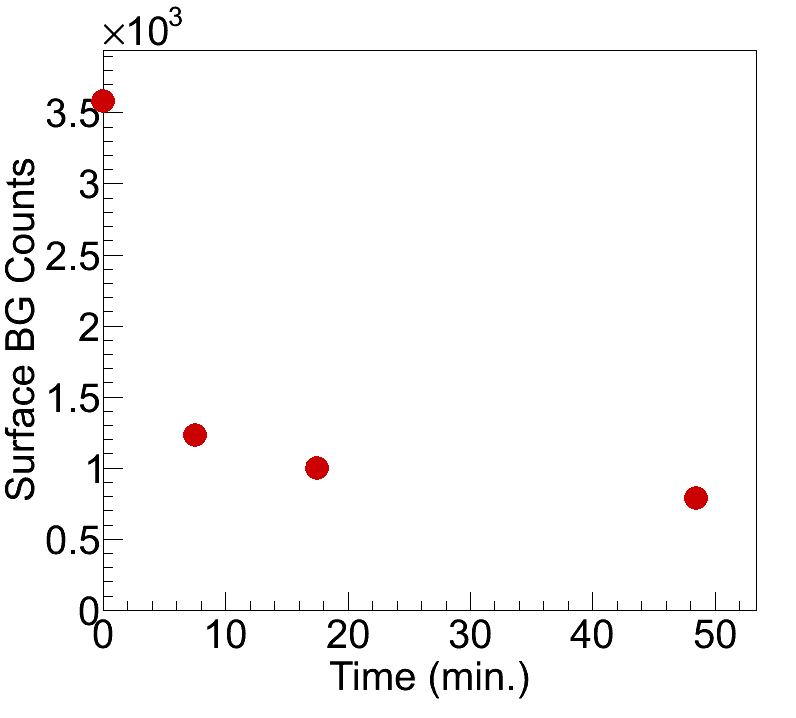
\includegraphics[width=.4\textwidth]{figures/Bleach_SurfaceBG_20150807_part1_vsTime.png}
                \caption{Decay of surface background emission during pre-bleaching of the sapphire window.}
\label{fig:surfBGbleach}
\end{figure}

\begin{figure} %[H]
        \centering
                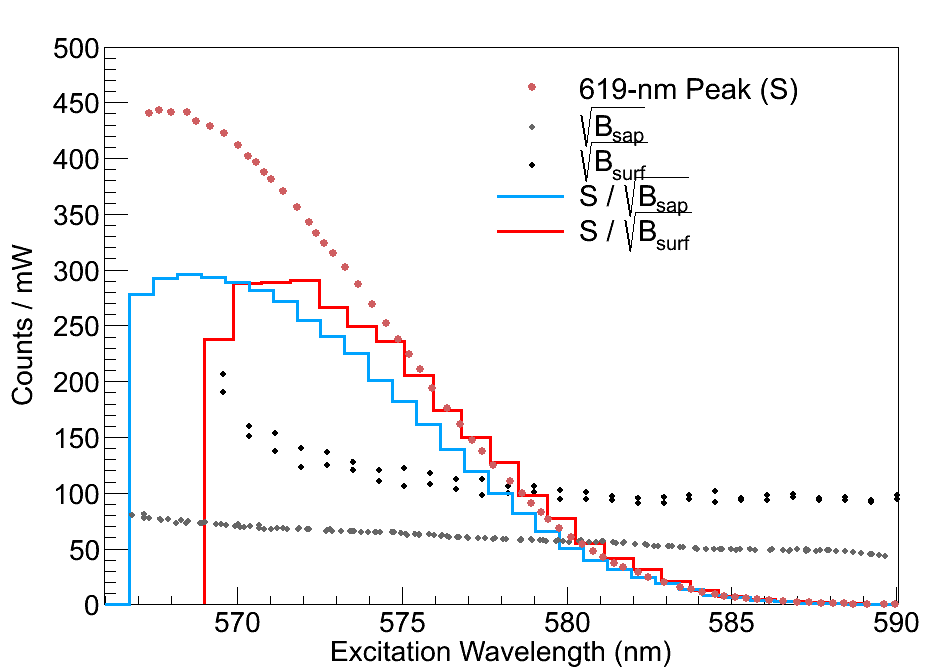
\includegraphics[width=.7\textwidth]{figures/S_to_B_both.png}
                \caption{Optimization of signal to background with the 619-nm fluorescence signal (S) for emission from the surface background (B$_{\text{surf}}$, red) and for the bulk sapphire emission (B$_{\text{sap}}$, cyan).}
        \label{fig:StoB}
\end{figure}

Consideration of signal-to-background ($S$/$\sqrt{B}$) guided the choice of 570~nm for excitation of the 619-nm fluorescence.  The signal, background, and $S$/$\sqrt{B}$ for emission passed by the 620-nm band-pass filter is plotted vs. excitation wavelength in Fig. \ref{fig:StoB} for both the surface background (B$_{\text{surf}}$) and the sapphire bulk emission (B$_{\text{sap}}$).  The peak in $S$/$\sqrt{B}$ represents the optimal excitation wavelength respective to each of the two background sources.  Around 568.5~nm is optimal vs. the sapphire emission, and around 571~nm is optimal vs. the surface background emission. 570~nm, which was used in sensitive imaging experiments, is nearly optimal in both cases, although 572~nm could have been used because the bulk sapphire background contribution was small in these experiments.